\documentclass[12pt,a4paper]{article}
\usepackage{amsmath,amssymb,mathrsfs,tikz,times,pifont}
\usepackage{enumitem}
\newcommand\circitem[1]{%
\tikz[baseline=(char.base)]{
\node[circle,draw=gray, fill=red!55,
minimum size=1.2em,inner sep=0] (char) {#1};}}
\newcommand\boxitem[1]{%
\tikz[baseline=(char.base)]{
\node[fill=cyan,
minimum size=1.2em,inner sep=0] (char) {#1};}}
\setlist[enumerate,1]{label=\protect\circitem{\arabic*}}
\setlist[enumerate,2]{label=\protect\boxitem{\alph*}}
%%%::::::by chnini ameur :::::::%%%
\everymath{\displaystyle}
\usepackage[left=1cm,right=1cm,top=1cm,bottom=1.7cm]{geometry}
\usepackage{array,multirow}
\usepackage[most]{tcolorbox}
\usepackage{varwidth}
\tcbuselibrary{skins,hooks}
\usetikzlibrary{patterns}
%%%::::::by chnini ameur :::::::%%%
\newtcolorbox{exa}[2][]{enhanced,breakable,before skip=2mm,after skip=5mm,
colback=yellow!20!white,colframe=black!20!blue,boxrule=0.5mm,
attach boxed title to top left ={xshift=0.6cm,yshift*=1mm-\tcboxedtitleheight},
fonttitle=\bfseries,
title={#2},#1,
% varwidth boxed title*=-3cm,
boxed title style={frame code={
\path[fill=tcbcolback!30!black]
([yshift=-1mm,xshift=-1mm]frame.north west)
arc[start angle=0,end angle=180,radius=1mm]
([yshift=-1mm,xshift=1mm]frame.north east)
arc[start angle=180,end angle=0,radius=1mm];
\path[left color=tcbcolback!60!black,right color = tcbcolback!60!black,
middle color = tcbcolback!80!black]
([xshift=-2mm]frame.north west) -- ([xshift=2mm]frame.north east)
[rounded corners=1mm]-- ([xshift=1mm,yshift=-1mm]frame.north east)
-- (frame.south east) -- (frame.south west)
-- ([xshift=-1mm,yshift=-1mm]frame.north west)
[sharp corners]-- cycle;
},interior engine=empty,
},interior style={top color=yellow!5}}
%%%%%%%%%%%%%%%%%%%%%%%

\usepackage{fancyhdr}
\usepackage{eso-pic}         % Pour ajouter des éléments en arrière-plan
% Commande pour ajouter du texte en arrière-plan
\usepackage{tkz-tab}
\AddToShipoutPicture{
    \AtTextCenter{%
        \makebox[0pt]{\rotatebox{80}{\textcolor[gray]{0.7}{\fontsize{5cm}{5cm}\selectfont PGB}}}
    }
}
\usepackage{lastpage}
\fancyhf{}
\pagestyle{fancy}
\renewcommand{\footrulewidth}{1pt}
\renewcommand{\headrulewidth}{0pt}
\renewcommand{\footruleskip}{10pt}
\fancyfoot[R]{
\color{blue}\ding{45}\ \textbf{2024}
}
\fancyfoot[L]{
\color{blue}\ding{45}\ \textbf{Prof:M. BA}
}
\cfoot{\bf
\thepage /
\pageref{LastPage}}
\begin{document}
\renewcommand{\arraystretch}{1.5}
\renewcommand{\arrayrulewidth}{1.2pt}
\begin{tikzpicture}[overlay,remember picture]
\node[draw=blue,line width=1.2pt,fill=purple,text=blue,inner sep=3mm,rounded corners,pattern=dots]at ([yshift=-2.5cm]current page.north) {\begingroup\setlength{\fboxsep}{0pt}\colorbox{white}{\begin{tabular}{|*1{>{\centering \arraybackslash}p{0.28\textwidth}} |*2{>{\centering \arraybackslash}p{0.2\textwidth}|} *1{>{\centering \arraybackslash}p{0.19\textwidth}|} }
\hline
\multicolumn{3}{|c|}{$\diamond$$\diamond$$\diamond$\ \textbf{Lycée de Dindéfélo}\ $\diamond$$\diamond$$\diamond$ }& \textbf{A.S. : 2024/2025} \\ \hline
\textbf{Matière: Mathématiques}& \textbf{Niveau : T}\textbf{S2} &\textbf{Date: 09/12/2024} & \textbf{Durée : 4 heures} \\ \hline
\multicolumn{4}{|c|}{\parbox[c]{10cm}{\begin{center}
\textbf{{\Large\sffamily Devoir n$ ^{\circ} $ 1 Du 1$ ^\text{\bf er} $ Semestre}}
\end{center}}} \\ \hline
\end{tabular}}\endgroup};
\end{tikzpicture}
\vspace{3cm}

\section*{\underline{Exercice 1 :} $0,5 \times 8 = 4$ points}
\begin{enumerate}
\item Énoncer le théorème des valeurs intermédiaires.
\item Énoncer le théorème d’existence et d’unicité d’une solution.
\item Énoncer le théorème de l’inégalité des accroissements finis (IAF).
\item \(\text{Si }\lim_{x \to x_0} \frac{f(x) - f(x_0)}{x - x_0} = a \ (a \neq 0) \text{ alors ... }\)
\item \(\text{Si }\lim_{x \to x_0^-} \frac{f(x) - f(x_0)}{x - x_0} = +\infty \text{ alors ... }\)
\item \(\text{Si }\lim_{x \to x_0} \frac{f(x) - f(x_0)}{x - x_0} = 0 \text{ alors ... }\)
\item \(\text{Si }\lim_{x \to +\infty} f(x) =+\infty \text{ et }\lim_{x \to +\infty}\frac{f(x)}{x}=\beta \in\mathbb{R}^{*}\text{ et }\lim_{x \to +\infty}[f(x)-\beta x]=+\infty\text{ alors ...}\)
\item Si \(f\) est continue et strictement décroissante sur \( ]-\infty; b] \), alors \( f(]-\infty; b]) = ... \)
\end{enumerate}

\section*{\underline{Exercice 2 :} 4 points}

\begin{enumerate}
    \item Calculer les limites suivantes : \textbf{(3 × 1 pt)}
    \[
    \lim_{x \to 0} \frac{\sqrt{1+\sin x} - 1}{\sin 2x} \; ; \quad
    \lim_{x \to 0} \frac{\cos x - 1}{x^3 + x^2} \; ; \quad
    \lim_{x \to 1} \frac{\sqrt{x + 3} - \sqrt{5 - x}}{\sqrt{2x + 7} - \sqrt{10 - x}}.
    \]
    \item Donner les primitives des fonctions \(f\) et \(g\) respectivement sur \(\mathbb{R}\) et \(\mathbb{R} \setminus \{1; 2\}\). \textbf{(2 × 0,5 pt)}
    \[
    f(x) = (3x-1)(3x^2-2x+3)^3 \; ; \quad
    g(x) = \frac{1-x^2}{(x^3-3x+2)^3}.
    \]
\end{enumerate}

\section*{\underline{Problème :} 12 points}

\underline{\textbf{Partie A :}}

Soit \( f \) la fonction définie par :
\[
f(x) = x - 2 - \sqrt{x^2 - 2x}.
\]

\begin{enumerate}
\item  Déterminer \( D_f \). \hspace{1cm} \textbf{(0,5 pt)}

\begin{enumerate}
    \item Calculer \( \lim_{x \to +\infty} f(x) \) et \( \lim_{x \to -\infty} f(x) \). \hspace{1cm} (0,25 pt), \textbf{(0,5 pt)}
    \item Étudier la branche infinie de la courbe \( (C_f) \) au voisinage de \( -\infty \). \hspace{1cm} \textbf{(0,75 pt)}
    \item Étudier la branche infinie de la courbe \( (C_f) \) au voisinage de \( +\infty \). \hspace{1cm} \textbf{(0,75 pt)}
\end{enumerate}

\item Étudier la dérivabilité de la fonction \( f \) à droite de 2 et à gauche de 0, puis interpréter géométriquement les résultats obtenus. \hspace{1cm} \textbf{(2 pt)}

\begin{enumerate}
    \item Justifier la dérivabilité de la fonction sur \( ]-\infty, 0] \cup ]2, +\infty[ \), puis\\ montrer que pour tout \( x \in ]-\infty, 0[ \cup ]2, +\infty[ \) :
    \(
    f'(x) = \frac{\sqrt{x^2 - 2x} - (x - 1)}{\sqrt{x^2 - 2x}}.
    \)    \hspace{1cm} \textbf{(1,5 pt)}

    
    \item Montrer que : \( \forall x \in ]-\infty, 0], f'(x) > 0 \) et \( \forall x \in ]2, +\infty[, f'(x) < 0 \). \hspace{1cm} \textbf{(1 pt)}
    
    \item Dresser le tableau de variations de la fonction \( f \). \hspace{1cm} \textbf{(1,25 pt)}
\end{enumerate}

\item Tracer la courbe \( (C_f) \) dans un repère orthonormé \( (O, \vec{i}, \vec{j}) \). \hspace{1cm} \textbf{(1,25 pt)}

\underline{\textbf{Partie B :}}

On considère la fonction \( g \) la restriction de la fonction \( f \) sur \( [2, +\infty[ \) :

\begin{enumerate}
    \item Montrer que \( g \) admet une fonction réciproque \( g^{-1} \) définie sur un intervalle \( J \)\\ que l’on déterminera . \hspace{1cm} \textbf{(0,5 pt)}
    
    \item Calculer \( g^{-1}(2 - 2\sqrt{2}) \). (On donne : \( g(4) = (2 - 2\sqrt{2} \)). \hspace{1cm} \textbf{(0,75 pt)}
    
    \item Déterminer \( g^{-1}(x) \) pour tout \( x \in J \). \hspace{3cm} \textbf{(0,5 pt)}
    
    \item Tracer la courbe \( (C_{g^{-1}}) \) dans le même repère orthonormé \( (O, \vec{i}, \vec{j}) \). \hspace{2cm} \textbf{(0,5 pt)}
\end{enumerate}

\end{enumerate}
\section*{\underline{Correction :} 12 points}
\underline{\textbf{Partie A :}}

Soit \( f \) la fonction définie par :
\[
f(x) = x - 2 - \sqrt{x^2 - 2x}.
\]

\begin{enumerate}
\item  Déterminons \( D_f \). \hspace{1cm} \textbf{(0,5 pt)}
$ f \quad \exists \quad$ ssi  $x^2 - 2x \geq 0 $

Posons $x^2 - 2x \geq 0 =0$

$x^2 - 2x \geq 0 =0 \implies x=0 \textbf{ ou } x=2$

    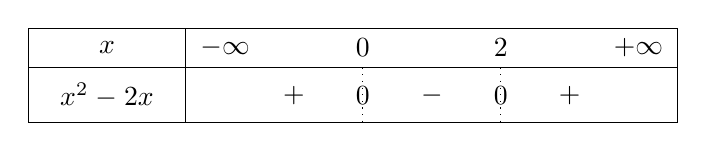
\begin{tikzpicture}[node style/.style={fill opacity=0,text opacity=1}]
        \tkzTabInit[espcl=1.75]{$x$/.5,$x^2 - 2x$/.7}{$-\infty$,$0$,$2$,$+\infty$}
        \tkzTabLine{,+,z,-,z,+,}
    \end{tikzpicture}

Donc $D_f=]-\infty ; 0] \cup [2 ; +\infty[ $

\begin{enumerate}
\item Les limites en $-\infty$ et en $+\infty$

\underline{en $-\infty$:}
\begin{align*}
\lim_{x \to -\infty} f(x) &= \lim_{x \to -\infty}x - 2 - \sqrt{x^2 - 2x}=-\infty
\end{align*}
\[
\textcolor{green}{\boxed{ \lim_{x \to -\infty} f(x) = -\infty  }} \textbf{ 0,25 points}
\]
\underline{en $+\infty$:}
\begin{align*}
\lim_{x \to +\infty} f(x) &= \lim_{x \to +\infty}x - 2 - \sqrt{x^2 - 2x}\\
													&= \lim_{x \to +\infty}\frac{(x - 2)^{2} - (x^2 - 2x)}{x - 2 + \sqrt{x^2 - 2x}}\\
													&= \lim_{x \to +\infty}\frac{x^{2}-2x+1 - x^2 + 2x}{x - 2 + \sqrt{x^2 - 2x}}\\
													&= \lim_{x \to +\infty}\frac{1}{x - 2 + \sqrt{x^2 - 2x}}\\
													&= 0
\end{align*}
\[
\textcolor{green}{\boxed{ \lim_{x \to +\infty} f(x) = 0  }} \textbf{ 0,25 points}
\]
\item La branche infinie de $(\mathcal{C}_{f}) $ en $-\infty$

Comme $\lim_{x \to -\infty} f(x) = +\infty$ Cherchons $\lim_{x \to -\infty} \frac{f(x)}{x}$
\begin{align*}
\lim_{x \to -\infty} \frac{f(x)}{x} &= \lim_{x \to -\infty}\frac{x - 2 - \sqrt{x^2 - 2x}}{x}\\
																		&=\lim_{x \to -\infty}\frac{x - 2}{x}-\frac{ \sqrt{x^2 - 2x}}{x}\\
																		&=1-\lim_{x \to -\infty}\frac{ \sqrt{x^2 - 2x}}{x}\\
																		&=1-\lim_{x \to -\infty}\frac{ -x\sqrt{1 - \frac{2}{x}}}{x}\\
																		&=1-\lim_{x \to -\infty}-\sqrt{1 - \frac{2}{x}}\\
																		&=0
\end{align*}
\textcolor{green}{Donc $(\mathcal{C}_{f}) $ admet une branche parabolique de direction $(oy)$ au voisinage de $-\infty$}
\item On a $\lim_{x \to -\infty} f(x)=0$
\textcolor{green}{Donc $y=0$  est A.H à $(\mathcal{C}_{f}) $ au voisinage de $-\infty$}
\end{enumerate}
\item Étudions la dérivabilité de la fonction \( f \) à droite de 2 et à gauche de 0, puis interprétons géométriquement les résultats obtenus. \hspace{1cm} \textbf{(2 pt)}\\
\underline{En $2^{+}:$}
\begin{align*}
\lim_{x \to 2^{+}} \frac{f(x)-f(2)}{x-2} &= \lim_{x \to 2^{+}}\frac{x - 2 - \sqrt{x^2 - 2x}}{x-2}\\
												&=\lim_{x \to 2^{+}} \frac{x - 2 }{x - 2 }-\frac{\sqrt{x^2 - 2x}}{x - 2 }\\
												&=1-\lim_{x \to 2^{+}}\frac{\sqrt{x^2 - 2x}}{x - 2 }\\
												&=1-\lim_{x \to 2^{+}}\frac{x(x - 2)}{ (x - 2)(\sqrt{x^2 - 2x}) }\\
												&=1-\lim_{x \to 2^{+}}\frac{x}{(\sqrt{x^2 - 2x}) }
\end{align*}
\[
\textcolor{green}{\boxed{ \lim_{x \to 2^{+}} f(x) =  -\infty }} \textbf{ 0,25 points}
\]
\textbf{Interprétation:} $f$ n'est pas dérivable en 0 mais admet au point $A(2;0=f(2))$ une demi-tangente verticale orientée vers le bas.

\underline{En $0^{-}:$}
\begin{align*}
\lim_{x \to 0^{-}} \frac{f(x)-f(2)}{x} &= \lim_{x \to 0^{-}}\frac{x - 2 - \sqrt{x^2 - 2x}+2}{x}\\
												&= \lim_{x \to 0^{-}}\frac{x - \sqrt{x^2 - 2x}}{x}\\
												&=\lim_{x \to 0^{-}} 1-\frac{\sqrt{x^2 - 2x}}{x}\\
												&=1-\lim_{x \to 0^{-}}\frac{\sqrt{x^2 - 2x}}{x}\\
												&=1-\lim_{x \to 0^{-}}\frac{x(x - 2)}{ x(\sqrt{x^2 - 2x}) }\\
												&=1-\lim_{x \to 0^{-}}\frac{(x - 2)}{\sqrt{x^2 - 2x}}
\end{align*}
\[
\textcolor{green}{\boxed{ \lim_{x \to 0^{-}} f(x) =  +\infty }} \textbf{ 0,25 points}
\]
\textbf{Interprétation:} $f$ n'est pas dérivable en 0 mais admet au point $A(0;-2=f(0))$ une demi-tangente verticale orientée vers le bas.
\begin{enumerate}
    \item Justifions la dérivabilité de la fonction sur \( ]-\infty, 0[ \cup ]2, +\infty[ \)\\
    
$ x \mapsto x - 2 $ est dérivable sur $\mathbb{R}$, comme fonction polynome, en particulier sur \( ]-\infty, 0[ \cup ]2, +\infty[ \)

$ x \mapsto - \sqrt{x^2 - 2x}$ est dérivable sur \( ]-\infty, 0[ \cup ]2, +\infty[ \), comme fonction irrationnelle

Par somme, $ x \mapsto x - 2 - \sqrt{x^2 - 2x}$ est dérivable sur \( ]-\infty, 0] \cup ]2, +\infty[ \).

Montrons que pour tout \( x \in ]-\infty, 0[ \cup ]2, +\infty[ \) :
    \(
    f'(x) = \frac{\sqrt{x^2 - 2x} - (x - 1)}{\sqrt{x^2 - 2x}}.
    \)    \hspace{1cm} \textbf{(1,5 pt)}
    
En effet $f(x)=x - 2 - \sqrt{x^2 - 2x}$

$f'(x)=1 - \frac{2x-2}{2\sqrt{x^2 - 2x}}=1 - \frac{x-1}{\sqrt{x^2 - 2x}}=\frac{\sqrt{x^2 - 2x}-(x-1)}{\sqrt{x^2 - 2x}}$
\item Montrons que : \( \forall x \in ]-\infty, 0], f'(x) > 0 \) et \( \forall x \in ]2, +\infty[, f'(x) < 0 \). \hspace{1cm} \textbf{(1 pt)}

Le signe de $f'$ dépend du numérateur.

Supposons que $\sqrt{x^2 - 2x} - (x - 1) <0 $

$$
\sqrt{x^2 - 2x} - (x - 1) <0 \implies \sqrt{x^2 - 2x} < (x - 1) \implies 
\begin{cases}
x^2 - 2x\geq 0 \\
x - 1 \geq 0 \\
x^2 - 2x < (x - 1)^{2}
\end{cases}
\implies 
\begin{cases}
x^2 - 2x\geq 0 \\
x - 1 \geq 0 \\
0 < 1
\end{cases}
$$

$$
\text{Posons }
\begin{cases}
x^2 - 2x = 0 \\
x - 1 = 0
\end{cases}
\implies
\begin{cases}
x=0 \text{ ou } x=2 \\
x = 1
\end{cases} 
$$

\begin{center}
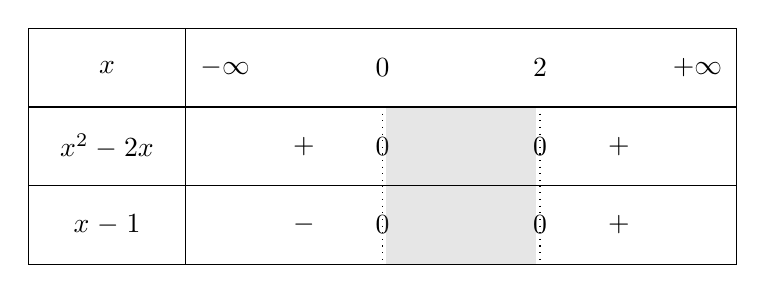
\begin{tikzpicture} 
\tkzTabSetup[doubledistance = 2pt,
             tstyle         =  dotted,
             hopacity       =.2,
             hcolor         = red!50!black]
\tkzTabInit[lgt=2,espcl=2] 
{
$x$ /1, 
$x^2-2x$ /1, 
$x-1$/1,
/0}% 
{$-\infty$ ,$0$ ,$2$ ,$+\infty$}% 
\tkzTabLine{ , + , z , h , z , + }
\tkzTabLine{ , - , z , h , z , +}
\end{tikzpicture} 
\end{center}
\begin{center}

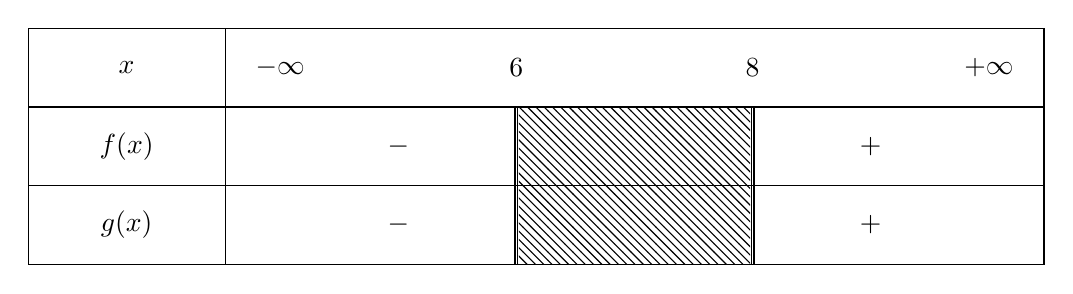
\begin{tikzpicture}
   \tkzTabInit[lgt = 2.5, espcl = 3, deltacl = 0.7]{$x$ / 1 , $f(x)$ / 1 , $g(x)$ / 1 }{$-\infty$, $6$, $8$, $+\infty$}
   \tkzTabLine{, -, d, h, d, +, }
   \tkzTabLine{, -, d, h, d, +, }
\end{tikzpicture}

\end{center}
Donc pour que $\sqrt{x^2 - 2x} - (x - 1) <0 $ il faut que $x\in ]2, +\infty[$

Ainsi, si $x\in ]-\infty, 0[$ alors $\sqrt{x^2 - 2x} - (x - 1) > 0 $

Donc \( \forall x \in ]-\infty, 0], f'(x) > 0 \) et \( \forall x \in ]2, +\infty[, f'(x) < 0 \)

\item Dressons le tableau de variations de la fonction \( f \). \hspace{1cm} \textbf{(1,25 pt)}

\begin{center}
    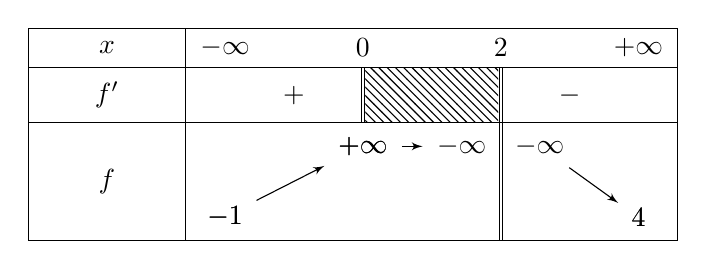
\begin{tikzpicture}[node style/.style={fill opacity=0,text opacity=1}]
        \tkzTabInit[espcl=1.75]{$x$/.5,$f'$/.7,$f$/1.5}{$-\infty$,$0$,$2$,$+\infty$}
        \tkzTabLine{,+,d,h,d,-,}
        \tkzTabVar{-/$-1$, +/$+\infty$, +D+/$-\infty$, -/$4$} 
    \end{tikzpicture}
\end{center}
\begin{center}
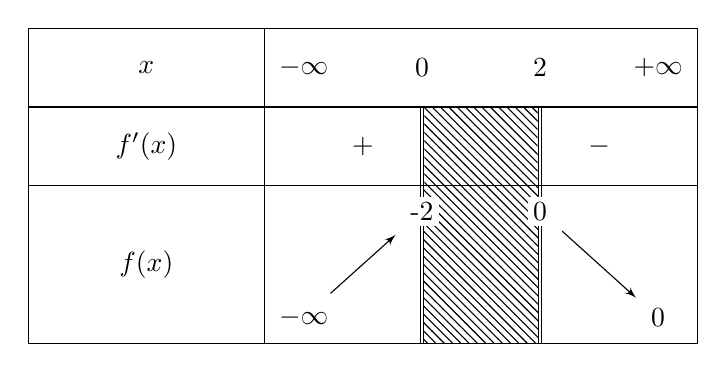
\begin{tikzpicture}
   \tkzTabInit[lgt=3,espcl=1.5]
     {$x$ / 1 , $f'(x)$ / 1, $f(x)$ / 2 }
     {$-\infty$, $0$, $2$, $+\infty$}
   \tkzTabLine
     { , + , d , h , d, -, }
   \tkzTabVar
   	{ -/$-\infty$ , +CH/-2, +C/0, -/0}
    %{ -/1 , +DH/$+\infty$, -C/0, +/1}
\end{tikzpicture}
\end{center}
\end{enumerate}
\begin{figure}[h]% Forcer l'image à cet endroit
\centering
\includegraphics[width=0.8\textwidth]{DevoirCurve.png}
\caption{Courbe de (Cf)}
\label{fig:monimage}
\end{figure}
\end{enumerate}

\end{document}
